\documentclass[11pt,a4paper]{article}
\usepackage[utf8]{inputenc}
%\usepackage[catalan]{babel}
\usepackage{comment}
\usepackage{pbox}
\usepackage{adjustbox}
\usepackage{amsmath}
\usepackage{amsfonts}
\usepackage{amssymb}
\usepackage[official]{eurosym}
\usepackage{graphicx}
\usepackage{fancyhdr}
\usepackage{appendix}
\usepackage{subfig}
\usepackage{xcolor}
\usepackage[ampersand]{easylist}
\usepackage{multirow}
\usepackage[hidelinks]{hyperref}
\usepackage[left=2cm,right=2cm,top=2cm,bottom=2cm]{geometry} 

\begin{document}
\begin{titlepage}

\begin{flushleft}
Escola Politècnica Superior\\
\vspace*{0.15in}
Master of Computer Engineering\\
\vspace*{0.15in}
ICT Project: Development and Implementation
\end{flushleft}

\begin{center}
\vspace{2.0cm}
\includegraphics[scale=0.3]{M-UdL.jpg}
\vspace{4.0cm}

\begin{LARGE}
\textbf{Sprint 2:}\\ 
\vspace*{0.15in}
\textbf{Requirement definition and system analysis}
\end{LARGE}
\vspace{5.0cm}

\vspace*{0.25in}
\textbf{Github: } \url{https://github.com/GarduinoTeam/Garduino}
\rule{80mm}{0.1mm}\\
\vspace*{0.1in}

\begin{large}
\textbf{Students:}

\begin{tabular}{ll}
Adrià Casals Espax  & Joan Pau Castells Gasia \\
Gerard Donaire Alos  & Roger Truchero Visa \\
\multicolumn{2}{c}{David Sarrat González}
\end{tabular}
\\
\vspace*{0.25in}
\textbf{Date:} \today \\
\end{large}

\end{center}
\end{titlepage}
 


\lhead[\thepage]{
\includegraphics[scale=0.05]{M-UdL.jpg}  }
\chead[]{\textbf{Automatic irrigation system with plague detection}}
\rhead[]{ICT Project}
\renewcommand{\headrulewidth}{0.5pt}
\renewcommand{\footrulewidth}{0.5pt}
\fancypagestyle{plain}{
\fancyhead[L]{}
\fancyhead[C]{}
\fancyhead[R]{\thepage}
\fancyfoot[L]{}
\fancyfoot[C]{}
\fancyfoot[R]{}
\renewcommand{\headrulewidth}{0pt}
\renewcommand{\footrulewidth}{0pt}
}
\pagestyle{fancy}
\vspace*{0.05in}

\tableofcontents

\newpage

\vspace*{0.3in}
\listoftables
\listoffigures
\newpage

\part*{Sprint 2}
\part*{Introduction}
\addcontentsline{toc}{part}{Introduction}
This document highlights the main advances and aspects of work relevant to the second sprint of the development of the Garduino project. 
\\ \\
This second iteration of the development of the project is mainly focused on the backend and frontend of the application, as well as the administration of users and the database. 
\\ \\
As such, the main aspects of the progress and changes in the project, as well as the requirements of the resulting sprint, product backlog and sprint backlog will be presented. 
\\ \\
As a result of this sprint, the general architecture of the application, a database model and a navigation scheme of the different screens and their internal relationship will be presented, both for the part of the web application and for the part of the Android application. Finally, it will offer a greater degree of deepening in financial factors and economic feasibility study.
\section{Software Installation}
\begin{itemize}
    \item Android Studio 3.5.2
    \item JBOSS with WildFly 10.0
    \item Pgadmin 4
    \item PostgreSQL 12.0.1
    \item Arduino 1.8.9
\end{itemize}

%% User stories
\begin{table}[htbp]
\centering
\begin{adjustbox}{angle=90,width=4.5in}
\begin{tabular}{|l|l|l|p{6cm}|l|l|}
\hline
\textbf{Id} & \textbf{As a} & \textbf{I want to be able to} & \textbf{So that} & \textbf{Priority} & \textbf{Sprint} \\
\hline \hline
1 & Administrator & Create, modify and delete devices & I can properly configure my irrigration system as a whole & HIGH & 2 \\
\hline 
2 & Administrator & Enable and disable devices & I can properly coordinate the different devices in my ittigation system at each time & MEDIUM & 2 \\
\hline
3 & Administrator & Create, modify and delete rules & I can properly set up the behavior of each device & HIGH & 2 \\
\hline
4 & Administrator & Enable or disable rules & I can perform punctual changes to the devices’ behavior at a certain moment & MEDIUM & 2 \\
\hline
5 & Administrator & Create, modify and delete conditions & I can customize and set up what each rule stands for in a high depth level & HIGH & 2 \\
\hline
6 & Administrator &  Enable or disable conditions & I can perform punctual changes to the rules’ definition at a certain moment & MEDIUM & 2 \\
\hline
7 & Administrator & Request the system to start and cancel manual irrigations for a device & I can order the system to start an immediate irrigation in a device regardless of the configuration and whether the expected conditions are being met & LOW & 2 \\
\hline
8 & Administrator & see the current real-time status of my device & I can keep track of each part of my irrigation system and my garden as a whole & HIGH & 2 \\
\hline
\end{tabular}
\end{adjustbox}
\caption{Table of user stories Sprint 2}
\end{table}

\newpage

\section{Product backlog + Sprint backlog}
\begin{figure}[hbtp]
\centering
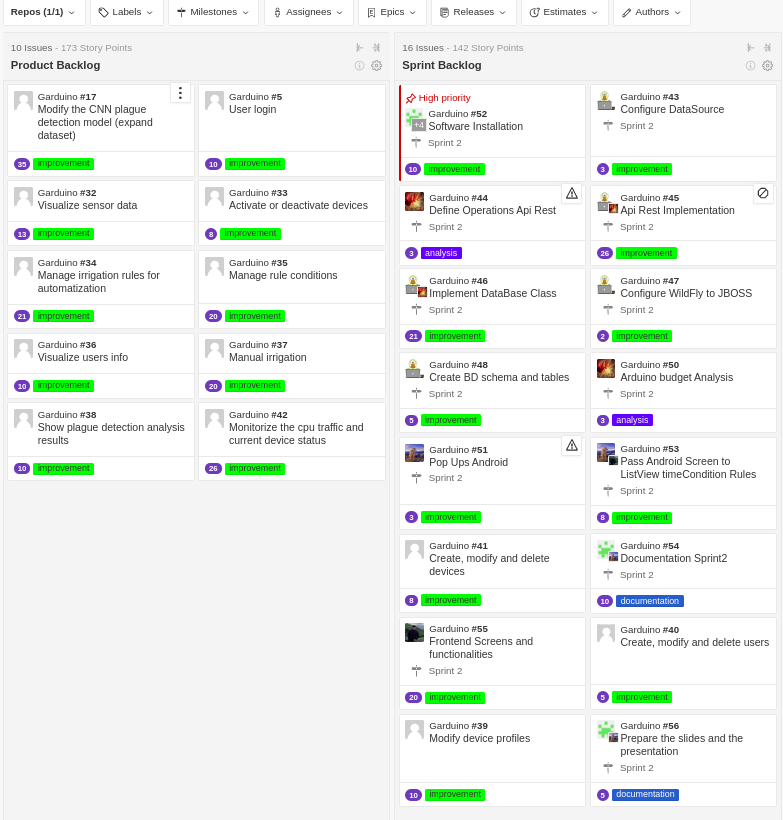
\includegraphics[scale=0.6]{Sprint2.png}
\caption{Product backlog and sprint backlog issues}
\end{figure}
\newpage
%% \section{Sprint backlog + dedication to each one}
%% Sprint backlog + dedication to each one
\begin{table}[htbp]
\begin{tabular}{|l|l|l|l|} 
\hline
Event                                                & Trigger     & Priority & Weight \\ \hline \hline
Modify the CNN plague detection model (expand dataset) & Users       & LOW     & 35  \\ \hline
User Login                                             & Users       & LOW   & 10  \\ \hline              
Visualize sensor data                                & Users/Admin & MEDIUM   & 13     \\ \hline
Enable or disable devices                            & Users       & MEDIUM   & 8      \\ \hline
Manage irrigation rules for automatization           & Users       & HIGH   & 21      \\ \hline
Manage rule conditions                               & Users       & HIGH   & 20     \\ \hline
Visualize users info                                 & Admin       & LOW      & 10     \\ \hline
Manual irrigation                                    & Users       & MEDIUM   & 20     \\ \hline
Show plaged detection analysis results               & Users       & MEDIUM   & 10     \\ \hline
Monitorize the cpu traffic and current device status & Admin       & MEDIUM   & 26     \\ \hline
Modify and list own devices                          & User        & MEDIUM   & 8      \\ \hline
Create, modify, delete, list own rules               & User        & MEDIUM   & 8      \\ \hline
Create, modify, delete, list own condition rules     & User        & MEDIUM   & 8      \\ \hline
\end{tabular}
\caption{Product Backlog explicit table}
\end{table}
The following issues have been added to the Product Backlog for the Sprint 3: 
\begin{itemize}
    \item Create, modify, delete, list own devices
    \item Create, modify, delete, list own rules
    \item Create, modify, delete, list own condition rules
\end{itemize}
\begin{table}[htbp]
\begin{tabular}{|l|l|l|l|} 
\hline
Event                                                & Trigger     & Priority & Weight \\ \hline \hline
Software Installation                                & Users       & HIGH     & 10     \\ \hline
Configure DataSource                                 & Users       & MEDIUM   & 10     \\ \hline
Define Operations Api Rest                           & Users       & LOW      & 10     \\ \hline
Api Rest Implementation                              & Users/Admin & MEDIUM   & 26     \\ \hline
Implement DataBase Class                             & Users       & MEDIUM   & 8      \\ \hline
Configure WildFly to JBOSS                           & Users       & MEDIUM   & 2      \\ \hline
Create DB Schema and Tables                          & Users       & MEDIUM   & 20     \\ \hline
Arduino Budget Analysis                              & Admin       & LOW      & 10     \\ \hline
Pop Up Screens Android                               & Users       & MEDIUM   & 20     \\ \hline
Pass Android Screen TimeConditionRules to ListView   & Users       & MEDIUM   & 10     \\ \hline
Create, modify, delete, list users                   & Admin       & MEDIUM   & 5      \\ \hline
Create, modify, delete, list devices                 & Admin       & MEDIUM   & 5      \\ \hline
Frontend screens and functionalities                 & Admin       & MEDIUM   & 5      \\ \hline
Create, modify, delete, list rules                   & Admin       & MEDIUM   & 5      \\ \hline
Create, modify, delete, list condition rules         & Admin       & MEDIUM   & 5      \\ \hline
Documentation Sprint 2                               & Team        & HIGH     & 21     \\ \hline
Prepare the slides and the presentation              & Team        & HIGH     & 8      \\ \hline
\end{tabular}
\caption{Sprint 2 Backlog explicit table}
\end{table}

\newpage
\section{Requirements}
\subsection{Non-functional requirements}
\begin{enumerate}
\item \textbf{Product}
	\begin{enumerate}
	
	\item \textbf{Accessibility and Usability}
		\begin{enumerate}
		\item Regardless of the style of interaction, the interface has to be simple and intuitive, providing a high level of interactivity and usability. The tasks will be as visual as possible, since the application will be oriented to all types of age ranges. 
		\end{enumerate}
	\item \textbf{Concurrency}
		\begin{enumerate}
		\item  The app has to be multi-user, allowing the usage of several users simultaneously of the application.
		\end{enumerate}
		
	\item \textbf{Portability}
		\begin{enumerate}
		\item \textbf{Adaptability (multi-device):} It is required that the design is "responsive" in order to ensure proper display on multiple devices, such as tablets, smartphones...
		\end{enumerate}
		
	\item \textbf{Support}
		\begin{enumerate}
		\item The mobile app will be developed by the Android platform.
		\end{enumerate}
	\end{enumerate}

\item \textbf{External}
	\begin{enumerate}
	\item \textbf{Privacy} 
		\begin{enumerate}
		\item All data management has to conform to the requirements of the organic law of data protection in order to preserve privacy in the processing of personal data.
		\end{enumerate}
		
	\end{enumerate}

\end{enumerate}

\subsection{Functional requirements}
\subsection{List of functionalities and features}
\textit{List of functionalities and features that all services (Android app, web service and Irrigation System) will accomplish}

\subsubsection{Android app}
\begin{itemize}
\item \textbf{The Android app will have to} allow communication with the web service.

\item \textbf{The Android app will have to} allow each user to log in.

\item \textbf{The Android app will have to} allow each user to configure/create an irrigation unit independently.

\item \textbf{The Android app will have to} show all irrigation units configured by the user.

\item \textbf{The Android app will have to} allow the manual watering option for each watering unit.

\item \textbf{The Android app will have to} allow planned irrigation of each irrigation unit.

\item \textbf{The Android app will have to} allow the option of monitoring the crop with data obtained from sensors and the webcam.

\item \textbf{The Android app will have to} allow the change of language.
\end{itemize}

\subsubsection{Web service}
\begin{itemize}
\item \textbf{The web service will have to} allow communication with the Android application and the Arduino devices.

\item \textbf{The web service will have to} allow the execution of a cron to make requests to the Arduino every X time so that a user can automatically receive notifications of his crop.

\item \textbf{The web service will have to} allow the execution of a machine learning script in charge of pest detection and return the data back to the Android application.

\item \textbf{The web service will have to} be able to determine when watering is optimal (if the automatic watering function has been used without programming) and send the request to the Arduino.

\item \textbf{The web service will have to} allow CRUD operations directly from the DB.
\end{itemize}

\subsubsection{Detection plague script}
\begin{itemize}
\item \textbf{The pest detection algorithm will have to}, using an image of a plant as an input, determine if is contaminated or not.
\end{itemize}

\begin{itemize}
\item RPi(\textbf{R}aspberry \textbf{Pi}) 3B (master):
	\begin{itemize}
	\item \textbf{The RPi will have to} allow communication with the web service.
	\item \textbf{The RPi will have to} send/receive data from/to the slaves to perform operations.
	\end{itemize}

\item NodeMCU ESP8266 (slave):
	\begin{itemize}
	\item \textbf{The NodeMCU will have to} be able to send the data to the RPi. 
	\item \textbf{The NodeMCU will have to} recolect the data from the humidity, temperature and soil sensors.
	\item \textbf{The NodeMCU will have to} capture and image of the device plant.		
	\item \textbf{The NodeMCU will have to} control the relay to make irrigation when receives the request from the RPi.
	\end{itemize}
\end{itemize}

\subsection{Observations}
\begin{itemize}
\item The leaf trimming algorithm requirement has been removed because the system will have a model that will already have the capabilities to process the whole image of the plant without the need of trimming it
\item The arduino/rpi architecture has been replaced by a master/slave architecture using RPi like a master and NodeMCU slaves.
\end{itemize}

\newpage

\section{Main use cases}
\begin{figure}[hbtp]
\centering
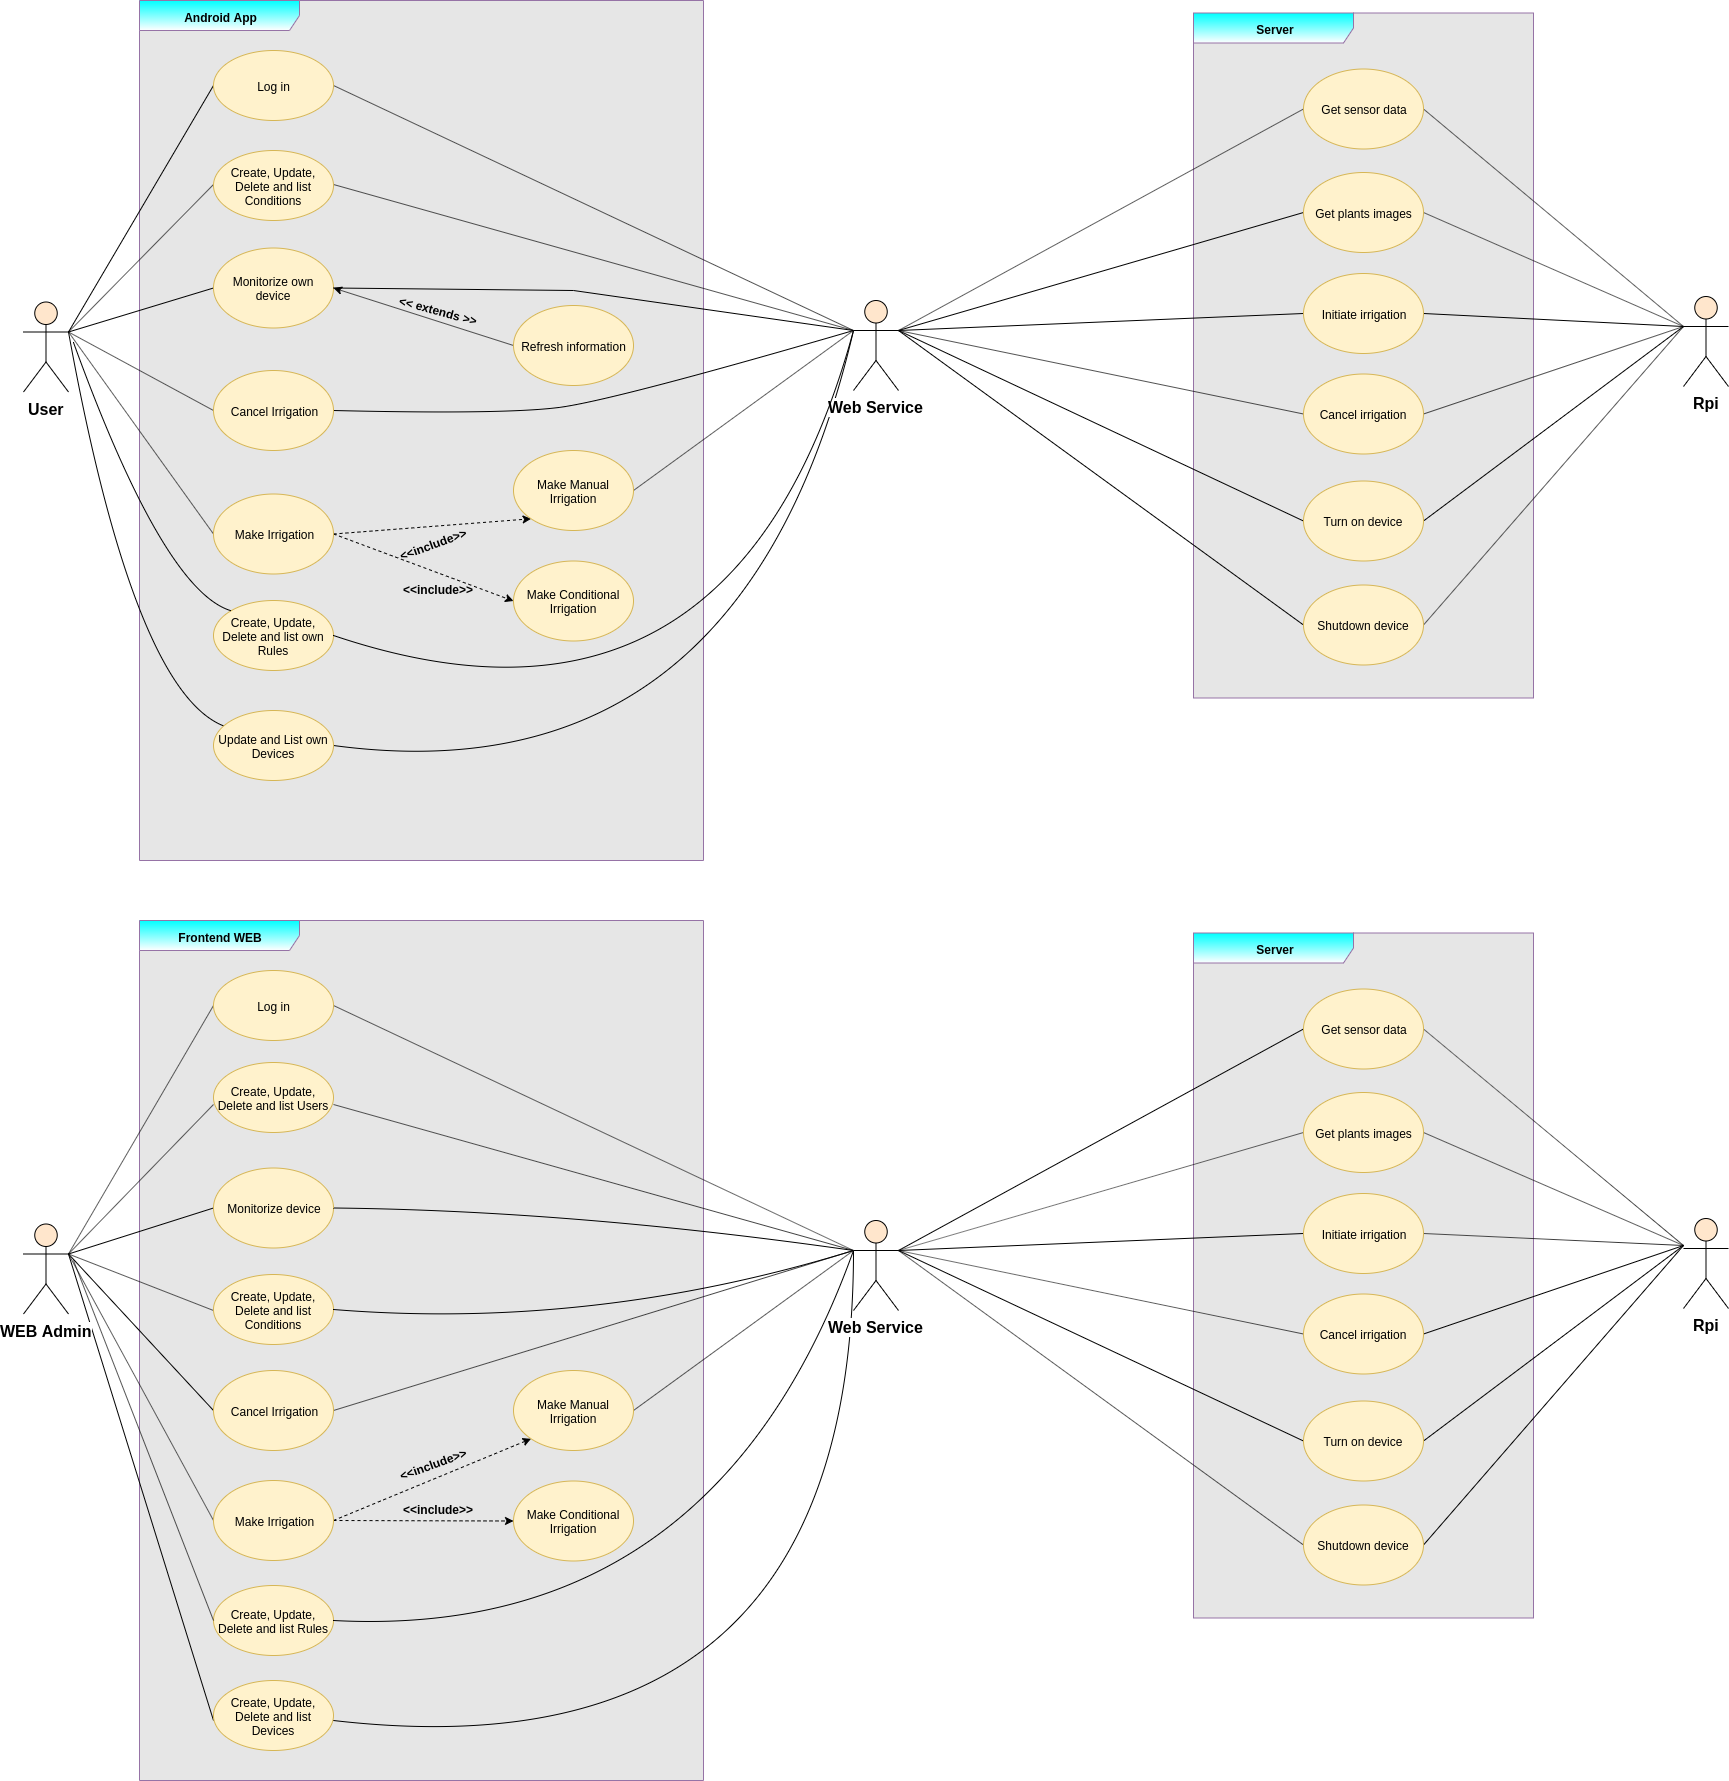
\includegraphics[scale=0.300,angle=0,origin=c]{DCU.png}
\caption{Application use cases diagram}
\label{figure2}
\end{figure} \newpage\leavevmode \\
 Figure \textcolor{blue}{ \ref{figure2}} shows the following actors: the user, the web service, the Rpi and the Admin.\newline\newline
The user will be able to log in, ask for their installations to be shown and edit them. He can also monitor his own installations. They can also create, modify, delete and list both their rules and irrigation conditions. In order to irrigate, the user will be able to irrigate their facilities manually and with irrigation conditions. All these functionalities are received by the Web Service which will wait for the requests that are made from the Android application and this one will ask for the necessary information to the Rpi to be able to give this information to the Android part and consequently to show it. \newline\newline
The admin will be able to logge, request that all the installations are shown as well as to create them, to modify them and to eliminate them. He can also monitor them. You can then create, modify, delete and list all rules, irrigation conditions and users. In order to water, the admin will be able to water all installations manually and with watering conditions. All these functionalities are received by the Web Service which will wait for the requests that are made from the frontend of the web part and it will request the necessary information to the Rpi to be able to give this information to the part of the frontend and consequently to show it.   
\newpage

\section{General architecture}
\subsection{System architecture}
\begin{figure}[hbtp]
\centering
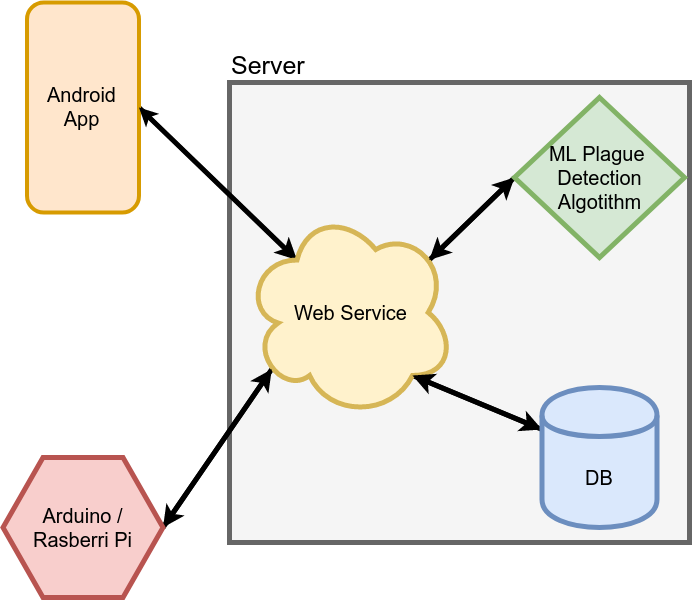
\includegraphics[scale=0.6]{AppArchitecture.png}
\caption{System app architecture}
\end{figure}

The architecture of our application is composed by:
\begin{itemize}
\item \textbf{Android App}: Graphical interface, in charge of collecting the data entered by the user. We are doing it using Android Studio.
\item \textbf{Web Service}: Makes middleware of the application. It manages requests between the Android app and the RPi/NodeMCU, the database, the frontend ...
\begin{itemize}
    \item \textbf{Frontend:} Graphical interface used by the web application administrator to perform operations against the backend of the webservice and monitor the status of each user's devices, thus allowing absolute control of the data to be given to the administrator.
    \item \textbf{Backend:} It is in charge of communicating with the android application, frontend and Rpi, receiving your requests, processing the data and preparing a response. It will act as the middleware of our system and therefore, will have more computational load.
\end{itemize}
\item \textbf{RPi/NodeMCU}: Device that will be in charge of the irrigation of each environment (gardening, flowerpot, ...).
\item \textbf{Database}: Manage all the data of the application, user credentials, register all requests, device info, ... 
\end{itemize}

\newpage

\subsection{RPi/NodeMCU architecture}
\begin{figure}[hbtp]
\centering
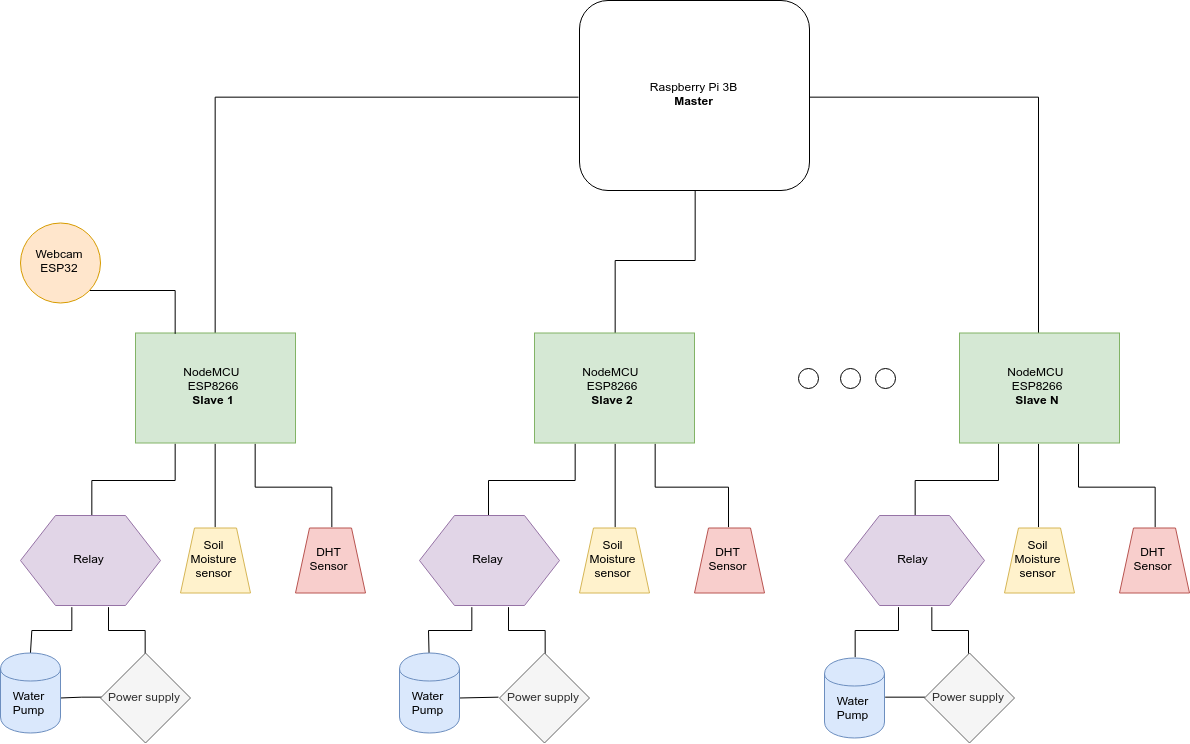
\includegraphics[scale=0.4]{IrrigationSystem.png}
\caption{Arduino and rapsberry pi architecture}
\end{figure}


So, we have the following components
\begin{itemize}
\item \textbf{Raspberry pi 3B}: We will use this microprocessor to ask the slaves for information about the sensors and the webcam, and then return the call to the web service with all the data.

\item \textbf{NodeMCU ESP8266}: It will act as a device slave, in charge of collecting sensor data, activating irrigation and capturing our plant. This microcontroller will have a wifi module to maintain a wireless communication with the RPi(\textbf{R}aspberry \textbf{Pi}).

\item \textbf{Webcam ESP32}: This module will be in charge of capturing the plant and sending the data to your NodeMCU.

\item \textbf{Relay}: Useful to control a motor, a led strip, or any other module using arduino. The use is sumple, just connect a digital output of our esp8266 to our relay module, and then we can control a power-demanding appliance with the digital signal provided by the esp8266.

\item \textbf{Water pump}: He will be in charge of pumping the water in order to carry out the irrigation correctly.

\item \textbf{Power supply}: Our devices will need a source of energy, in this case we have chosen a power supply of 12V to batteries. In the future it could be exchanged for a solar panel or even make a hybrid between the two depending on the climate.

\item \textbf{Soil moisture sensor}: Measures the volumetric water content in soil. Since the direct gravimetric measurement of free soil moisture requires removing, drying, and weighing of a sample, soil moisture sensors measure the volumetric water content indirectly by using some other property of the soil, such as electrical resistance, dielectric constant, or interaction with neutrons, as a proxy for the moisture content.

\item \textbf{DHT sensor}: This sensor will allow us to simultaneously measure temperature and humidity. We have two types of DHT sensors, DHT11 and DHT22.\\

The DHT11 is a very limited sensor that we can use for training, testing, or in projects that don't really require accurate measurement.\\

The DHT22 has acceptable features for use in real monitoring or logging projects that require medium accuracy.\\ 

In this project we will start implementing the DHT11 version due to its low cost (70 cents).
\end{itemize}

\newpage

\section{Data model}
%% Data model
\begin{figure}[hbtp]
\centering
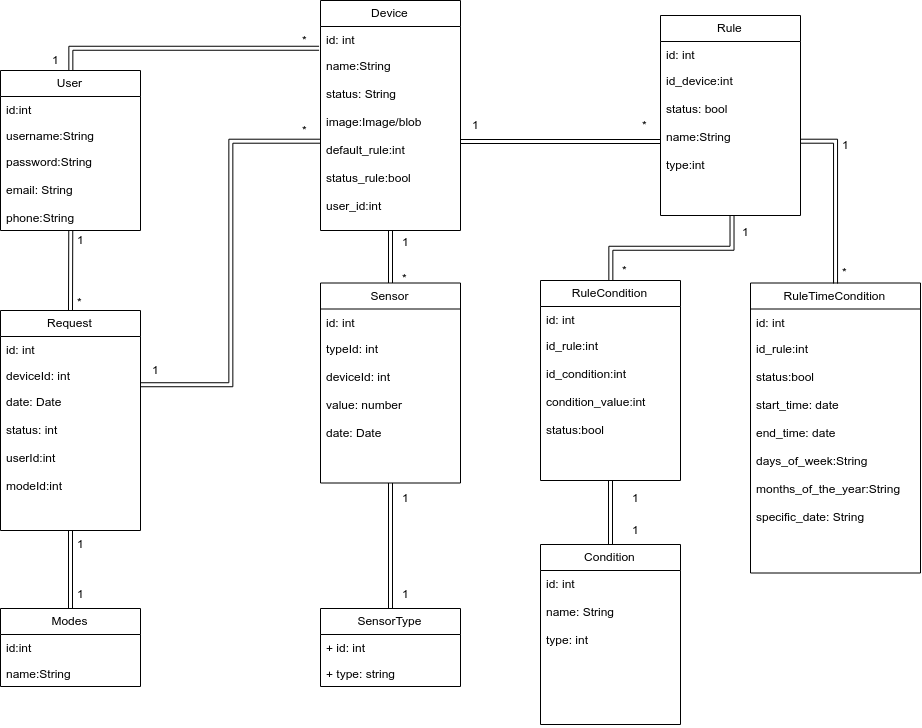
\includegraphics[scale=0.5]{ModelDeDades.png}
\caption{Data model UML}
\end{figure}
In this data model diagram we can see how our data is structured and related with the different datatables. We explain the target of the different tables:

\begin{itemize}
\item \textbf{User}: It stores all the data related to our users.

\item \textbf{Request}: It is used to store the requests of the users  to a specific device and to check if these requests have been completed. 

\item \textbf{Mode}: It stores the different kind of requests that a user can do  like manual irrigations, conditional irrigations, the obtainment of the sensor data.

\item \textbf{Device}: It stores the information of a device which corresponds to a user. It can have a default rule, so the user has not need to create its own. 

\item \textbf{Sensor}: It stores the value of a sensor of a specific type which correspond to a device.

\item \textbf{SensorType}: It stores the different type of sensors which are: Humidity, Temperature, Soil.

\item \textbf{Rule}: It stores all the configurations which correspond to a device. It can have RuleConditions and TimeConditions.

\item \textbf{RuleCondition}: It stores the conditions  with its respective value. It corresponds to a rule and a condition. If the sensors data of a device accomplish these conditions then an irrigation is produced.  

\item \textbf{RuleTimeCondition}: It corresponds to the conditions of a rule which a user decides when an irrigation has to be produced.  With the status we determine if this condition has to be considered.

\item \textbf{Condition}: It stores the different conditions which are: Temperature is lower than,Temperature is greater than, Humidity is lower than,  Humidity is greater than, Soil is lower than, Soil is greater than.
\end{itemize}

We have made some changes regarding the data model of the previous sprint in:
\begin{itemize}
    \item \textbf{User Table:} An admin field has been added to distinguish between normal and admin users.
    \item \textbf{Device Table:} Image field has been removed since the Web Service use a file system storage to store the images of the devices. For example, to create a new device for a user with id=1 with name device 1 the path would be: \{ServerHome\}/1/device1.png.
    \item \textbf{ status\_rule} and \textbf{default\_rule} were not necessary since the satus of a rule is controlled yet and the \textbf{default\_rule} is the type of a User Rule or Admin Rule.
    \item \textbf{SensorType Table:} The field type is now the name field.
    \item \textbf{Condition Table:} The field type was not used.
    \item \textbf{RuleTimeCondition Table:} The specific\_dates field is now an array of dates.
\end{itemize}
\newpage

\section{Main screens desgin and Navigation}
%% Navigation schema between activities
\begin{itemize}
\item Link Android Design:\newline\newline \textcolor{blue}{\href{https://drive.google.com/file/d/1GWvJHmUxLQVg-ns894TZreQi0Cy9rv79/view?usp=sharing}{Click here: Android Screens Navigation}}

\item Brief explanation of the different screens in the Android application: 
\\ \\
On screen 1, a list of the different devices available in the user's installation is shown. You can see the last photograph taken by the system, as well as the last date and time of irrigation. As such, the user can activate and deactivate the system for that particular device by means of a switch, or enter the panel of that particular device by pressing on the rest of the box pertinent to that device. 
\\ \\
Screen 2 shows the control panel for a particular device. The last image obtained by the system, temperature, humidity and soil can be consulted. 
You can see the last time and date the data was updated. A manual irrigation can be started and the configuration of the device can be accessed.
\\ \\
Screen 3 shows the pop-up relevant to the operation of a manual irrigation. You can enter a numerical amount on how long the irrigation will last, and you are given the option of initializing the irrigation or canceling it.
\\ \\
Screen 4 shows the control panel of a device when there is a manual irrigation in progress. It indicates how much irrigation time is left, and offers the option of cancelling it instantaneously. 
\\ \\
Screen 5 shows the configuration menu of a device. It offers the option to change its name, change the frequency of updating information and access to a panel to modify the irrigation rules. All changes will be saved when you press the save button. 
\\ \\
Screen 6 shows the configuration panel of a device's irrigation ruleset. It shows the list of rules, which can be activated and deactivated by means of a switch, and these can be modified by clicking on them. It shows the option to add new rules and the option to save changes.
\\ \\
Screen 7 shows the irrigation rule creation screen. You can choose its name, confirm its creation and cancel it. This screen will be converted to a pop-up in the near future of the development of the project. 
\\ \\
Screen 8 shows the configuration panel of the irrigation rules of a device after a new irrigation rule has been created. The internal configuration of this can now be accessed and modified by clicking on its name. 
\\ \\
Screen 9 shows the configuration panel of an irrigation rule. This will consist of various conditions, which can be activated and deactivated through the use of a switch. It offers the option to modify the parameters of the conditions, as well as to create a new one and save the changes in that irrigation rule. 
\\ \\
Screen 10 shows the screen to add a new condition. It shows the different types of conditions that are available. 
\\ \\
Screen 11 shows the configuration of a time condition. It shows the various options for which the condition will be active: start and end time of the days it will be active, configuration by days of the week, by months in which it will be active, and specific dates in which the time condition will be active. 
\\ \\
Screen 12 shows the modification of one of the parameters related to the time of a time condition (start time and end time). The specific times can be selected by specifying them in a clock. 
\\ \\
Screen 13 shows the modification of the parameters relative to the specific dates in which the time condition will operate. The specific days can be chosen by means of a calendar. 
\\ \\
As an improvement of the previous prototype, some screens have been changed by the pop-ups corresponding to these in order to streamline navigation and maintain an awareness of the location between the various screens on which the user navigates at all times. 

\item Link Web Design:\newline\newline
 \textcolor{blue}{\href{https://drive.google.com/file/d/1_nxHsY7jSMUKHQmlxoCyGm_XgQ5xAlk8/view?usp=sharing}{Click here: Web Screens Navigation}}
 \item Brief explanation of the different screens in the Web application: 
\\ \\
Screen 1 shows information about the statistics of our application like RPI petitions, available server ram, cpu, ...
\\ \\
Screen 2 shows the control panel in order to list, create, edit or eliminate users.

\\ \\
Screen 3 shows the control panel related to the operation of creating a user. Admin have to enter: user name, email, password and phone.
\\ \\
Screen 4 shows the control panel related to the operation of editing a user account. Admin can modify whatever he wants (username, email, password and phone). 
\\ \\
Screen 5 shows the control panel related to the devices for each user in order to list, create, edit or eliminate devices. 
\\ \\
Screen 6 shows the control panel related to the operation of creating a device.
\\ \\
Screen 7 shows the control panel related to the operation of editing a device.
\\ \\
Screen 8 shows the control panel related to the conditions of a rule in order to list, create, edit or eliminate conditions.
\\ \\
Screen 9 shows the control panel related to the operation of creating a condition.
\\ \\
Screen 10 shows the control panel in order to list, create, edit or eliminate rules.
\\ \\
Screen 11 shows the control panel related to the operation of editing a rule.
\\ \\
Screen 12 shows the control panel related to the operation of creating a rule.

\end{itemize}
\section{Financial Factors}
The financial factors analysis is present in the Market and economic study document.
\end{document}
